\documentclass[crop,tikz]{standalone}% 'crop' is the default for v1.0, before it was 'preview'
\usepackage{tikz,calc,pgfplots}
\usepackage{tikz-3dplot}
\usetikzlibrary{calc}
\usetikzlibrary{calc,patterns,decorations.pathmorphing,decorations.markings}
\usetikzlibrary{shapes.geometric}
\begin{document}

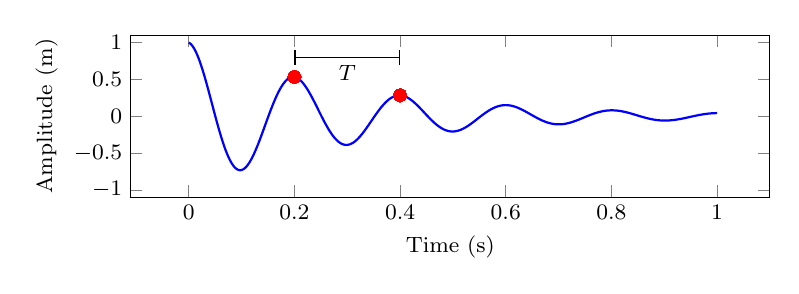
\begin{tikzpicture}[scale=1]
	\footnotesize
	\begin{axis}[
		width=0.8\textwidth,
		height=0.3\textwidth,
		xlabel={Time (s)},
		ylabel = {Amplitude (m)},
		xmax=1.1,
		ymax=1.1,
		ymin=-1.1,  
		samples=500]
		
		\def\wn{5*2*pi};
		\def\xo{1};
		\def\dxo{0};		
		\def\zeta{0.1};
		\def\wdd{sqrt(1-\zeta^2)*\wn};
		\def\phi{rad(atan(\dxo/(\wdd*\xo)))};
		
		
		\addplot[blue, thick, domain=0:1] (x, {sqrt(\xo^2+(\dxo/\wdd)^2) * cos(deg(\wdd*x- \phi)) * exp(-\zeta*\wn*x)});
		
		\addplot[red, mark=*, thick, domain=0:1] (0.2, {sqrt(\xo^2+(\dxo/\wdd)^2) * cos(deg(\wdd*0.2- \phi)) * exp(-\zeta*\wn*0.2)});
		\addplot[red, mark=*, thick, domain=0:1] (0.4, {sqrt(\xo^2+(\dxo/\wdd)^2) * cos(deg(\wdd*0.4- \phi)) * exp(-\zeta*\wn*0.4)});
		
		\draw [|-|] (axis cs: 0.2,0.8) -- (axis cs: 0.4,0.8)  node [below, pos=0.5] {$T$};
	\end{axis}
	
\end{tikzpicture}

\end{document}